\documentclass[12pt]{article}

% taken from APL Memo style
\topmargin      -1in 
\marginparsep   0in
\headheight     .75in  
\headsep        0.25in
\textheight     9in 
\oddsidemargin  0in 
\evensidemargin 0in 
\textwidth      6.50in 

\pdfoptionpdfminorversion=6

\usepackage[hyphens]{url}
\usepackage{hyperref}
\usepackage{subcaption}
\usepackage{fancyhdr}
\usepackage[usenames,dvipsnames]{color}
\usepackage{listings}  
\usepackage{cite}
\usepackage{graphicx}
\usepackage{mathptmx}
\usepackage{acronym}
\usepackage{array}
\usepackage{gensymb}
\usepackage[toc,page]{appendix}
\usepackage{color, colortbl}
\usepackage{multirow}
\usepackage{booktabs}
\usepackage{gensymb}
\usepackage[nottoc]{tocbibind}
\usepackage{hyperref}
\usepackage{cleveref}

\definecolor{Gray}{gray}{0.9}

\newcolumntype{L}{>{\centering\arraybackslash}m{3cm}}
\hypersetup{colorlinks=true, 
	 	    linkcolor=black, 
		    urlcolor=black, 
		    citecolor=black,
		    filecolor=black}
		    
\urlstyle{rm}

% add any other paths here where images might reside (ideally a relative path)
\graphicspath{ {images/} }

% for two-column references
% from: http://tex.stackexchange.com/questions/20758/bibliography-in-two-columns-section-title-in-one
%\usepackage{multicol}
%\usepackage{etoolbox}
%\patchcmd{\thebibliography}{\section*{\refname}}
%    {\begin{multicols}{2}[\section*{\refname}]}{}{}
%\patchcmd{\endthebibliography}{\endlist}{\endlist\end{multicols}}{}{}
\setlength{\parindent}{0in}

\acrodef{nlp}[NLP]{Natural Language Processing}
\acrodef{cnn}[CNN]{Convolutional Neural Network}
\acrodef{rnn}[RNN]{Recurrent Neural Network}
\acrodef{api}[API]{Application Programming Interface}
\acrodef{bow}[BOW]{Bag of Words}
%%% paragraph spacing
%\setlength{\parindent}{4em}
\setlength{\parskip}{1em}

\begin{document}
\begin{titlepage}
	\centering
	
\includegraphics[width=\textwidth]{jhu_logo.png}\par\vspace{2cm}
	{\scshape\Huge Application of Convolutional Neural Networks to Natural Language Processing \\
	\vspace{1.5cm}
	 \scshape\Large EN.525.801(21) - Special Project I Summer 2016\par}
	{\scshape \Large Austin Dress\par} 
	\vspace{0.75cm}
%	{\scshape \Large DRAFT\par}
	\vfill
	{\large \today\par}
\end{titlepage}

\tableofcontents
\listoftables

\newpage

\section{Preface} 
\ac{nlp} is a field in computer science that focuses on processing human language. Human language can be referred to as a natural language as it has evolved overtime without strict syntax rules that one would find in programming languages. A simple example of \ac{nlp} would be processing a sentence and identifying the verb, subject, adjective. Writing a program to process a scholarly article and generate a summary would be a more advanced application of \ac{nlp}.

In recent years \ac{cnn}s, a deep learning technique for image classification, have gained huge popularity after Alex Krizhevsky won the Imagenet LSVRC2012 competition with his network \cite{alex}. Since then \ac{cnn}s have shown promising results in many other domains such as audio processing and \ac{nlp}. 


Over the course of the semester I explored using Word2Vec \cite{word2vec} to create word embeddings and then train a \ac{cnn} on the embeddings for sentiment analysis of various datasets. This document captures topics in \ac{nlp} that I explored throughout the semester, and my classification results for two datasets.

\section{Development Schedule}

In \cref{App:AppendixA} the development schedule is shown for the semester. This chart was created as a way to set short term goals for the semester to keep myself on task. The semester is broken down into research, testing and evaluation, and finally documentation and presentation at the end of the semester. 

\section {Background and Previous Work}
Prior to beginning the semester I had very little experience with \ac{nlp} and thus needed to do some reading on how traditional classifiers are built for sentiment analysis. In this section I cover data preparation that is necessary in any \ac{nlp} task as well as two feature vector representations for language. When training a classifier for any type of task the input is usually a feature vector containing floating point numbers and integer labels. As a result words must be converted to a number representation. 

\subsection {Data Preprocessing and Cleaning}
Similar to image processing where a image may be preprocessed by convolving a gaussian kernel and normalizing the image, \ac{nlp} also has its own form of data preprocessing. Take for example the following tweets from the Sentiment140 dataset \cite{sentiment140}:

\begin{enumerate}
	\item \#poemsunder140 ....started by \@shannonelyse1
	\item Juuuuuuuuuuuuuuuuussssst Chillin!!
	\item :-D ))))))))...WHAT AN AMAZING NIGHT,DAY \&amp; NIGHT AGAIN!! HI TWITS! I MiSS U GUYS"
	\item @dandelionas is making fettucini and garlic bread!
\end{enumerate} 

Twitter tweets contain text fields known as ``hash tags", a phrase proceeded by a ``\#" symbol, and an ``at" symbol, a username proceeded by an ``@" symbol. Tweets 1 and 4 contain such information and for the purposes of sentiment analysis are extraneous as hastags and twitter usernames do not tend to appear or relate to sentiment. In addition, repeated letters in words, capitalization of entire words, punctuation marks, and emoticons are removed. Prior to being passed to a classifier for training or testing these tweets would be converted to the following (as an example): 

\begin{enumerate}
	\item started by
	\item just chillin
	\item what an amazing night day night again hit twits i miss u guys
	\item is making fettucini and garlic bread
\end{enumerate} 

This cleaning and preprocessing step is typically exploits regular expressions to quickly locate the patterns previously mentioned and remove them.

\subsection{Co-occurence Matrices}

One method for representing a word in a document in \ac{nlp} is to use use the surrounding words in a sentence to represent a word. This brought about the idea of the co-occurence matrix. This matrix captures the number of times a other word occurs directly next to it in a dataset. For example in the Standford Deep Learning Course \cite{dl_course}, they show the following example:

\begin{itemize}
	\item I like deep learning.
	\item I like NLP.
	\item I enjoy flying.
\end{itemize}

\begin{figure}[htbp!]
	\centering
	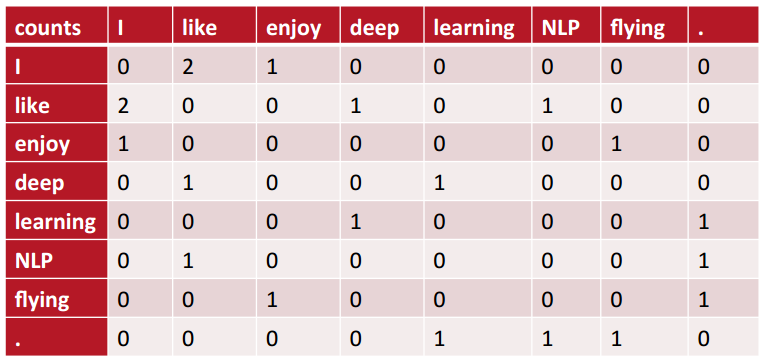
\includegraphics[scale=.4]{cooccurence.png}
	\caption{Co-occurence Matrix example.}
	\label{fig:cooccurence}
\end{figure}

This matrix shown in Figure \ref{fig:cooccurence} displays the number of times words appear next to each other in the three sentences above. The idea is that each row represents a feature vector that characterizes each word in the whole dataset.

There are obvious drawbacks to representing words in this way. One being that as the number of words in the dataset increases, so does the dimensionality of the matrix. Representing words in this way allows us to create a similarity metric between words as words in human language tend to appear next to each other. In Section \ref{word2vec} the Word2Vec word representation is covered. Word2Vec is a more state of the art word representation technique.

\subsection {Bag of Words}

The \ac{bow} algorithm is used in many \ac{nlp} applications such as sentiment analysis and also has applications in image processing. The general algorithm is described as it was used as a baseline for the two datasets used during the semester. The \ac{bow} algorithm and its word representation is  fairly intuitive. As an example take the common American English language tongue-twister and its response:

\begin{enumerate}
	\item How much wood could a woodchuck chuck if a woodchuck could chuck wood?
	\item A woodchuck would chuck as much wood as a wouldchuck could chuck if a woodchuck could chuck wood.
\end{enumerate} 

From these two sentences a vocabulary, or word corpus, can be built. For these two phrases the corpus would be: \{\textit{how, much, wood, could, a, woodchuck, chuck, if, would, as}\}.

\ac{bow} builds a feature vector for a sentence, paragraph, or document by counting the number of time a given word appears. For the two phrases listed above the feature vector representations would be as follows:

\begin{enumerate}
	\item \{1,1,2,2,2,2,2,1,0,0\}
	\item \{0,1,2,2,3,3,3,1,1,2\} 
\end{enumerate} 

One of the nice features of \ac{bow} is that the feature vectors produced by it are always the same length. The main downfall of the \ac{bow} is that as the corpus size increases so does the dimensionality of the feature vector. This results in feature vectors that are very sparse. For example, training \ac{bow} on the Twitter tweets would result in feature vectors with many zeros as tweets are limited to 140 characters. It is for this reason that a corpus size limit of, for example 5000 words is enforced. 

\section{Word2Vec} \label{word2vec}

Word2Vec \cite{word2vec} is an unsupervised learning technique for generating word embeddings developed in C++ by Google. Word2Vec is similar to co-occurence matrices previously mentioned, but produces very dense word vector representations. These word vectors contain rich information about how they relate to other words. This concept is similar to finding a strong correlation between neighbor pixels in an image. In the case of an image RGB values are known already. With sentences it's clear to a human that there is correlation between words in sentence, but it's not clear how to capture this information in a vector space. Word2Vec is one solution to this problem though there are others such as GloVe \cite{pennington2014glove} researched at Stanford.

Training a Word2Vec model is as simple as taking a text dataset, preprocessing it, and feeding the sentences into the training function. The Gensim \cite{rehurek_lrec} library was utilized to train and test Word2Vec models. Gensim is a Python wrapper around Google's C++ code that makes setting up data and training a model easier.

Prior to training a Word2Vec model Gensim requires that several parameters be set:

\begin{table}[!htbp]
	\centering
	\footnotesize
	\begin{tabular}{|>{\raggedright\arraybackslash}m{30mm}|m{70mm}|m{20mm}|m{20mm}|}
		\hline
		\rowcolor{Gray}
		\multicolumn{1}{|>{\centering\arraybackslash}m{30mm}|}{\textbf{Parameter}} 
		& \multicolumn{1}{>{\centering\arraybackslash}m{70mm}|}{\textbf{Description}} 
		& \multicolumn{1}{>{\centering\arraybackslash}m{20mm}|}{\textbf{Typical Value}}\\ \hline
		num\_features       & Word Vector Dimensionality & 300          \\ \hline
		min\_word\_count   &  Minimum number of times word must appear to be included & 40          \\ \hline
		context  & Context window Size     & 10     \\ \hline
		downsampling & Downsample setting for frequent words           & 1e-3           \\ \hline
	\end{tabular}
	\caption{Input parameters for training a Word2Vec model.}
	\label{table:gensim_inputs}
\end{table}

The values shown in Table \ref{table:gensim_inputs} are the main tunable parameters for the algorithm. In general 300 feature dimensions produces good results. The minimum word count is a good way to remove words that are misspelled. 

\begin{figure}[htbp!]
	\centering
	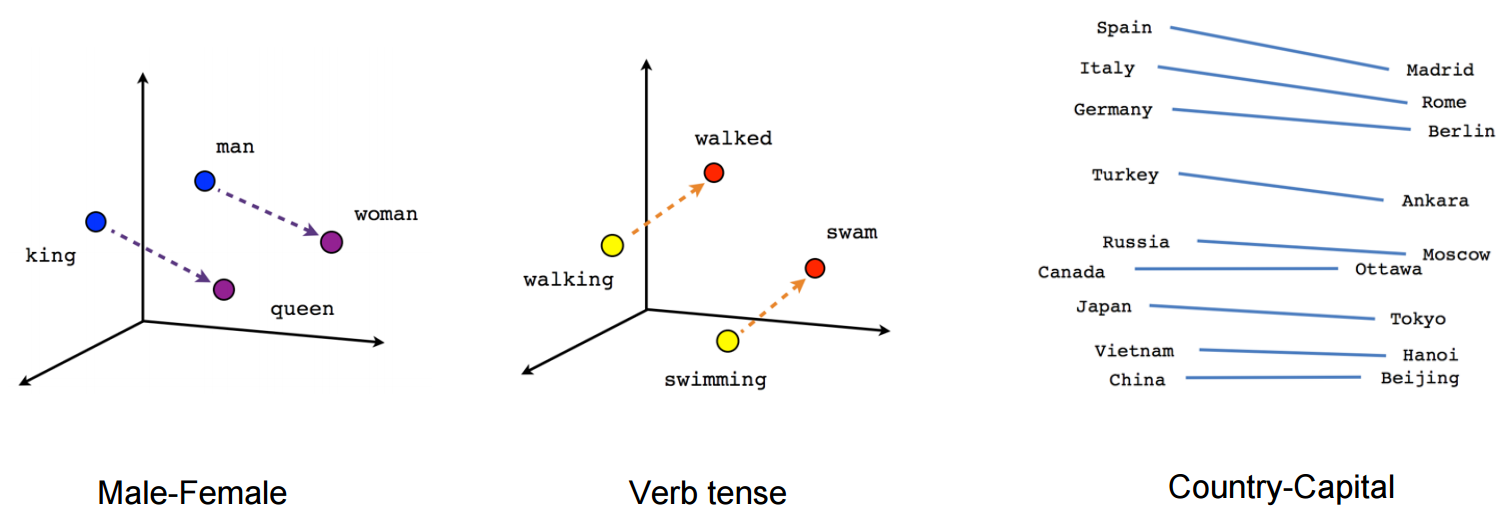
\includegraphics[scale=.3]{linear-relationships.png}
	\caption{Word vector visualization \cite{tensorflow} showing semantic relationships between words.}
	\label{fig:linear-relation}
\end{figure}

Figure \ref{fig:linear-relation} and Appendix \ref{App:AppendixB} show words plotted in feature space after dimension reduction and projection. These plots show the power of Word2Vec word embeddings as similar words are spatially close to each other. Performing vector addition and subtraction reveals interesting properties. Specifically the embeddings are able to capture analogies. Several Word2Vec models were trained throughout the semester. Below I show several screenshots of outputs from a model I trained.

\begin{figure}[htbp!]
	\centering
	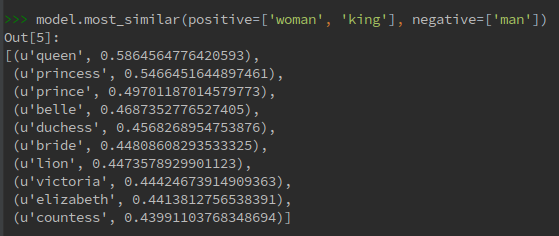
\includegraphics[scale=.5]{man_woman.png}
	\caption{Example of Word2Vec vector addition and subtraction.}
	\label{fig:man_woman}
\end{figure}

In Figure \ref{fig:man_woman} I demonstrate the following vector addition and subtraction: woman + king - man. The output of the model suggests the top 10 closest words in the vector space. Queen is the closest in the feature space and is likely the answer that human would give to this analogy.

\begin{figure}[htbp!]
	\centering
	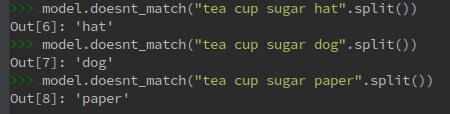
\includegraphics[scale=.5]{tea_cup.png}
	\caption{Word2Vec determining which word does not belong.}
	\label{fig:tea_cup}
\end{figure}

Related words are closely spaced in feature space which makes it possible to do other interesting tasks such as identifying words that do not belong in the same set/classification. Figure \ref{fig:tea_cup} shows that Word2Vec embeddings can correctly identify that the words \{hat, dog, paper\} do not belong to the same set of words \{tea, cup, sugar\}.


\section {Keras: Designing a CNN Network for Sentence Classification}
Keras \cite{chollet2015keras} is one of the many nerual network frameworks/libraries available for deep learning. Keras is very modular and supports \ac{cnn}s, \ac{rnn}s, and standard neural networks. Keras technically is a python wrapper around the Theano and TensorFlow deep learning frameworks. I decided to use this tool to construct \ac{cnn}s due to it's flexibility and rapid prototyping capability. Changing the number of filters in a \ac{cnn}, size, and\slash or number of fully connected layers is very simple. 

\begin{figure}[htbp!]
	\centering
	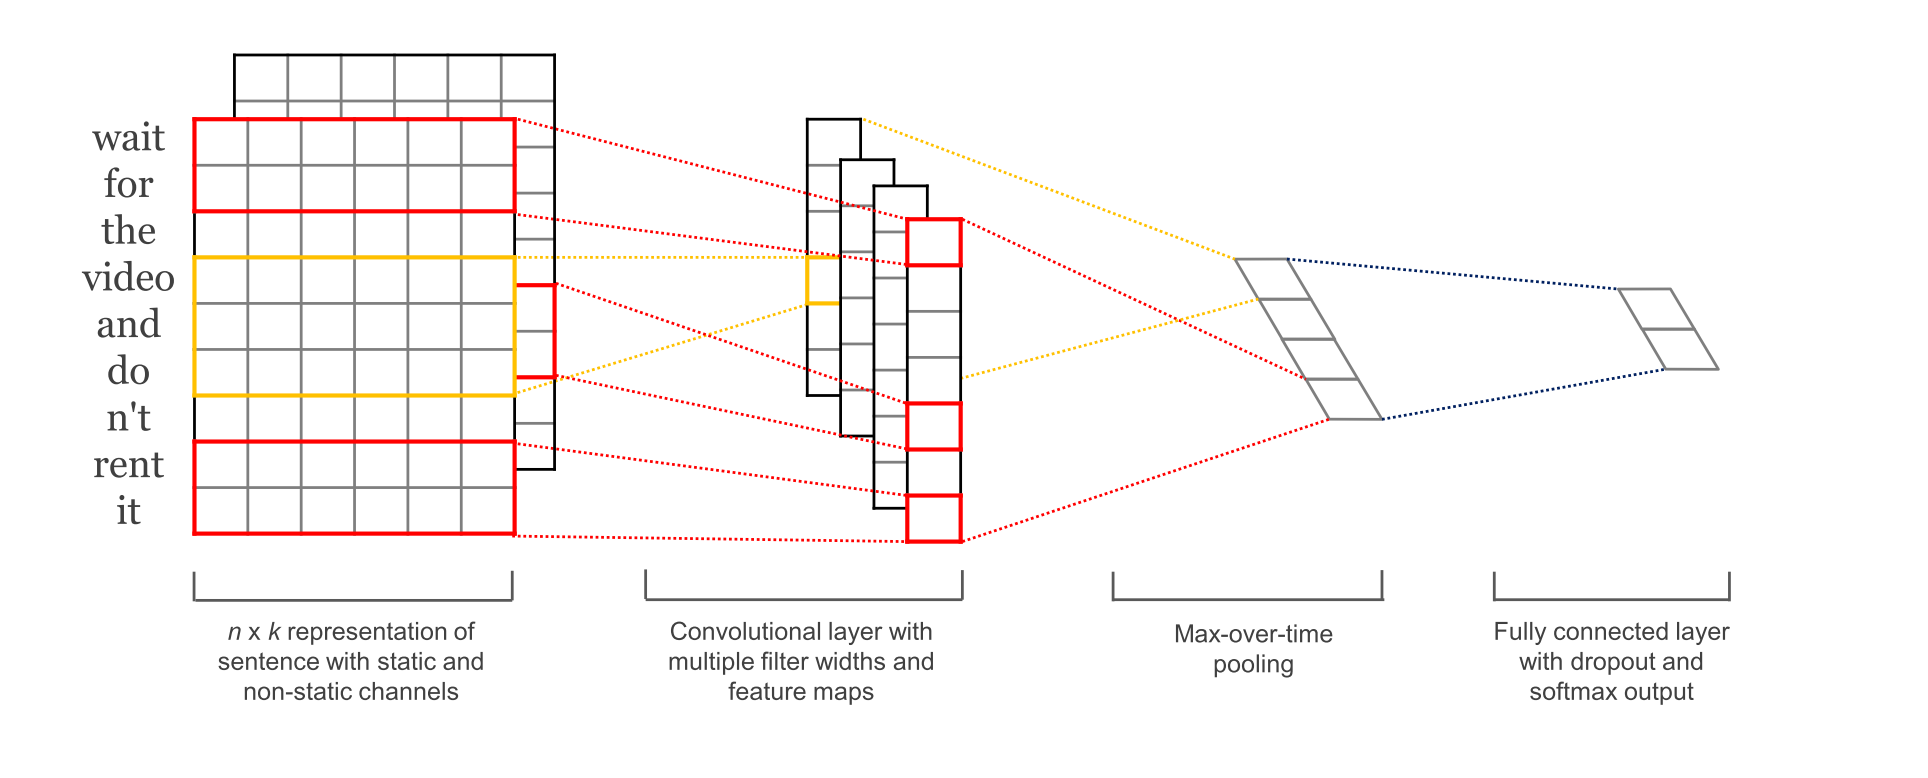
\includegraphics[scale=.4]{network_structure.png}
	\caption{Example \ac{cnn} architecture for sentence classification \cite{kim2014convolutional}.}
	\label{fig:network_structure}
\end{figure}

\begin{figure}[htbp!]
	\centering
	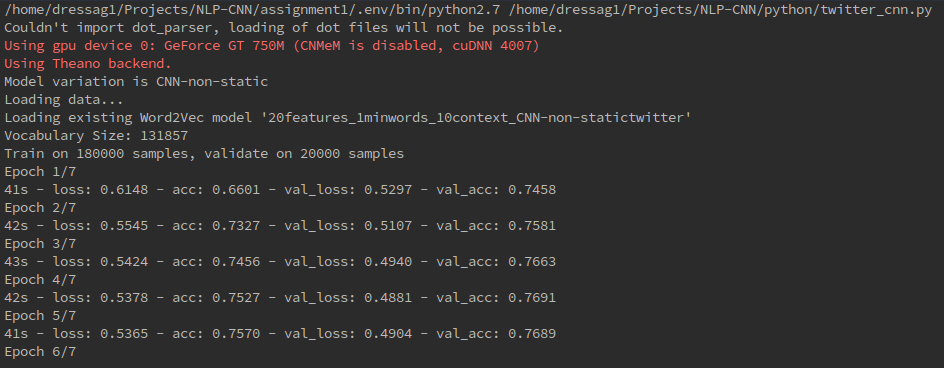
\includegraphics[scale=.4]{training.png}
	\caption{Output from Keras when training a \ac{cnn}.}
	\label{fig:training}
\end{figure}



\section{IMDB Movie Review Dataset}
Dataset came with training and testing sets already defined. In total for training there were 24722 labeled reviews, and for testing there were a similar number of 24723 reviews that are unfortunately unlabeled. This dataset was attained through a Kaggle Data Science Competition. The competition has since ended but the dataset is still available. Since the hosted data was for a competition, Kaggle only provided the labeled training set. For this reason, I had to split the data to make my own training and test sets. The data was split 80\slash20 for training and testing respectively.

pos train: 9873
neg train: 9905

neg test = 2444
pos test = 2500

train 18000, 2000 validation, 5000 test
Vocabulary size = 81322 words

accuracy:86.06 percent

Confusion Matrices
[[1897  581]
[ 116 2406]]

[[ 0.77  0.23]
[ 0.05  0.95]]


\section{Twitter Sentiment Dataset}

Twitter is a social networking website \cite{twitter} where users can post 140 character messages on their accounts. Once the message is posted it is completely open to the entire Twitter user base. Twitter has evolved as a means of rapidly sharing information and events. For example, a company may choose to post that a new product is available on Twitter in addition to their website to reach a larger user base. Twitter posts are rich with sentiment and make it a good source for sentiment analysis.

To date there are no large hand labeled twitter datasets available for sentiment analysis. This led several Stanford Researchers \cite{Go_Bhayani_Huang_2009} to collect and build their own dataset called Sentiment140 \cite{sentiment140}. Labeling individual tweets for sentiment is a very tedious task, so the authors came up with a very creative way to mine positive and negative tweets. Twitter data was collected through the Twitter \ac{api} and labeled by using positive and negative emoticons. For example, if a tweet included a smiley face ``:)" it was considered positive. If a tweet contained both a positive and negative emoticons the tweet was not used. The dataset was collected between April 6, 2009 to June 25, 2009.

In total there are 1.6 million tweets used for training. The number of positive and negative tweets are equal for train. The testing data is much smaller only containing 500 tweets. The tweets used for testing were hand labeled, where as the training tweets were mined.

Vocabulary Size 564692 words.
Max Sequence length was 52 words.

Based on paper Twitter Sentiment Classification using Distant Supervision \cite{Go_Bhayani_Huang_2009}. The dataset that they provide was

Used same CNN network structure \cite{kim2014convolutional}

after 7 epochs
rand - 78 %
cnn-non-static - 75 % 75.98 %
cnn- static

cnn-non-static on 359 test exemplars after 7 epochs
[[130  47]
[ 37 145]]

[[ 0.73  0.27]
[ 0.2   0.8 ]]

100 features
[[142  35]
[ 42 140]]
[[ 0.8   0.2 ]
[ 0.23  0.77]]


\newpage
\appendix
\section{\\Project Development Schedule} \label{App:AppendixA}
% the \\ insures the section title is centered below the phrase: AppendixA
\begin{figure}[htbp!]
	\centering
	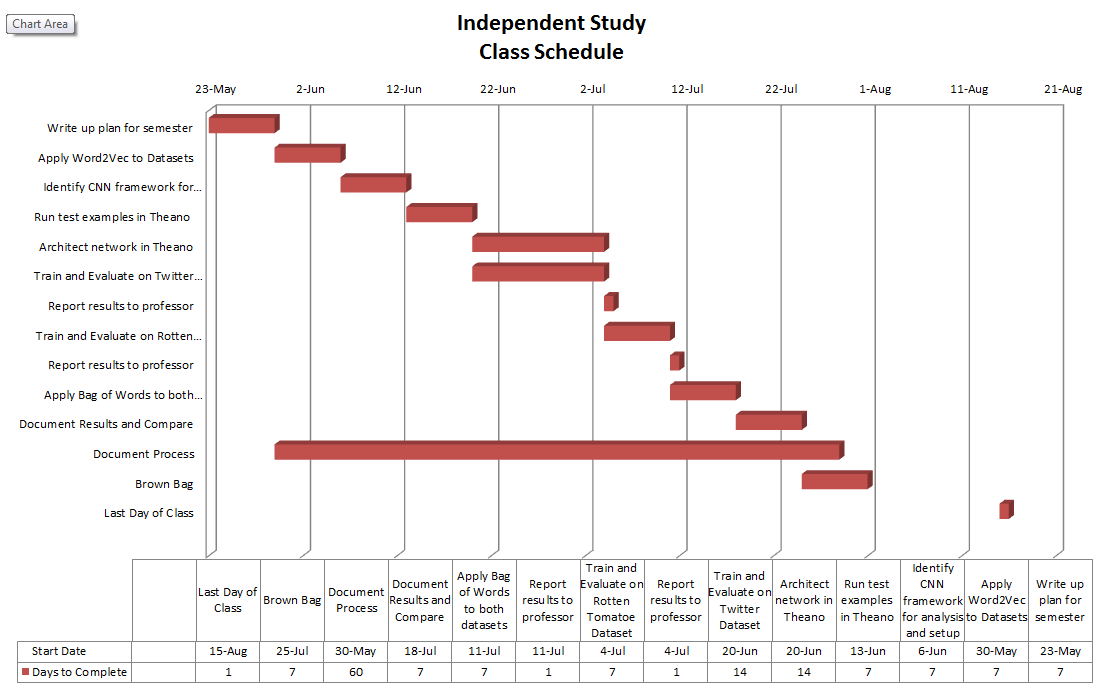
\includegraphics[scale=.5]{gantt.PNG}
	\caption{Project Development Schedule}
%	\label{fig:schedule}
\end{figure}

\newpage
\section{\\Word2Vec Feature Plot} \label{App:AppendixB}
% the \\ insures the section title is centered below the phrase: Appendix B

\begin{figure}[htbp!]\centering
	\centering
	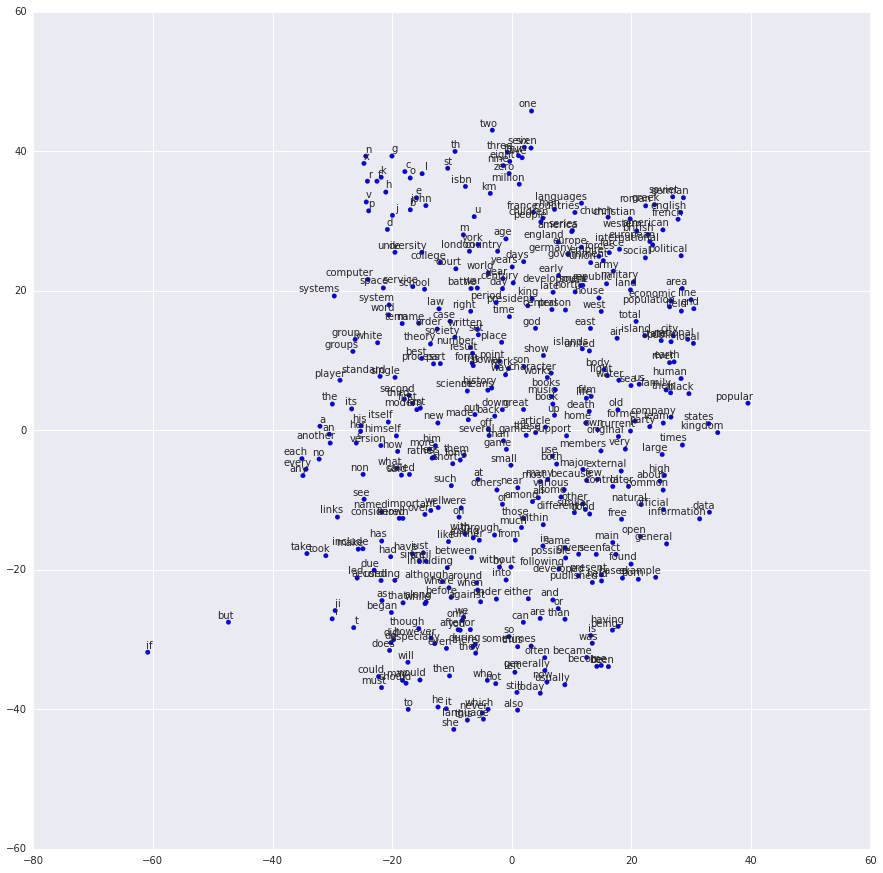
\includegraphics[scale=.5]{tsne.png}
	\caption{Word2Vec vector plot showing that similar words appear near each other in the feature space \cite{tensorflow}.}
	%	\label{fig:schedule}
\end{figure}

\newpage
\bibliography{Austin_Dress_NLP_CNN_Summer_2016.bib}
\bibliographystyle{plain}




\end{document}
